\section{Introduction}

This is an exploratory study of capital investment by public school districts responsible for providing K-12 education. Recent studies have found mixed results for the effect of capital spending on test scores- a presumed measure of output. \cite{biasi_what_2024} find positive productivity results, while \cite{cellini_value_2010} find no effects on children’s outcomes. \cite{jackson_what_2024} find that overall, capital spending and current spending have about equal returns. Our goal is to provide some perspective by which the effects of public capital can be studied. Specifically, if school districts are not on their production possibility frontier with capital, then it will not be possible, or useful, to measure the productivity of additional capital. Schools will not be on their productivity frontier if they have other objectives than those in the presumed output of the specified production function, which generally have been student test scores. Thus, we assemble evidence on the two primary choices facing school districts; one is the level of investment to reach the preferred level of capital stock, and the other is the method to finance the desired investment. We therefore subject data on school financing to five tests, with implications for evidence on potential objectives. First, we frame two tests over the smoothing of capital expenses over time and the business cycle, with a view towards equity of cohorts over time. We construct two additional tests by estimating an Error Correction Model (ECM), and investigating the relative importance of enrollment compared to income per capita and population. A final test estimates the ECM for two groups, school districts that borrow frequently and those that seldom borrow. The administrative structure exists so that variation in the frequency of borrowing should be irrelevant. On the other hand, if there are administrative elements that impact borrowing frequency, the level of capital stock may estimates but segments by the frequency of borrowing. looks to the relative importance of administrative criteria by specifying the capital stock as a function of the frequency of borrowing.

Our empirical tests combine a careful look at the data describing capital financing and expenditure by school district, as well as regression analysis using an Error Correction Model as indicated by our statistical tests. We look at school districts only in the large US metropolitan regions, so that the competitive environment in which districts find themselves is relatively similar. Further, our data focuses exclusively on independent school districts, which are those that have some ability to set their own tax rates and level of debt. Our data thus consists of a square panel containing financing and enrollment information from 2609 school districts from 58 MSAs, composed of 194 counties in 26 states. 

School districts presumably will choose the level of capital appropriate to achieving their objectives. The objective of school districts is not obviously clear. Were the objective to maximize the standardized test scores for students, then presumably the marginal impact of capital for new buildings, building maintenance, educational technology, plumbing, air conditioning, and even school buses should be equal per dollar of expenditure. On the other hand, were districts to have different attributes in their objective functions, factors outside the education production function might also be important. Simply as an example, if the goal of the district were to have as large as capital stock possible (a variant of budget maximization), then capital spending might be maximized given access to debt. Alternatively, if labor is disproportionately influential in the decision process, capital might have a lower or higher shadow price than labor in the production function. Our empirical examination provides evidence that other factors besides students are important to decisions concerning capital spending.

School districts have a much broader array of vehicles by which capital expenditures can be financed than for current expenditures. Unlike current spending, capital expenditure may be financed by debt\footnote{In theory, this might even be more efficient because the cost of capital will be spread over the users through debt service.}. One potential impact of debt is to make it administratively easier to smooth capital expenditures over time. Intertemporal equity across cohorts has recently been shown to be a relatively neglected topic in schools \cite{biolsi_inequality_2022}, a surprising condition given the attention that equity in education resources has garnered cross-sectionally. Capital spending can be smoothed over time not only because additional debt can be taken during periods of resource shortfalls, but school districts also have special saving funds, called bond funds, that can be accessed over time solely for capital spending. In contrast, current expenditures are subject to the balanced budget constraints where expenditures cannot exceed current revenues.

While capital expenditures can be undertaken with debt, districts also have the choice of paying for capital out of current resources. The data available from Census sources does not distinguish the source of financing for capital. We construct a measure of current financing of capital by subtracting from total capital expenditure changes in various aspects of the debt picture, and arrive at an estimate of about 67\% of capital being financed out of current resources. The practice may have advantages for smoothing expenditures over time, to the extent that capital expenditures formerly financed currently can be switched to debt financing in low resource periods, with debt picking up the displaced capital expenditures. 

To this time our first two tests about smoothing and alternative school district objectives constitute solely a look at the data. We show that there is a wide variety of debt behavior by school districts. Further, we find that the economic health of the economy as seen by recessionary periods does not appear to be motivating to changes in the financing structure. We do not find that there is an increase in debt during or just after recessions, when debt substitution out of current expenditures might be expected. We expect to be much more explicit about these issues in the next version of our paper.

The second pair of statistical tests for the presence of alternative objectives arises out of estimates of an Error Correction Model (ECM). We empirically analyze the importance of enrollment compared to variables that determine the tax base. While enrollment will change the costs facing a school district, income and population affect the tax base, as well as potentially demand, without changing the actual cost constraint. Thus we test whether income and population impact capital, and we test for the speed of adjustment of the capital stock when either enrollment, or the tax base, changes.

Our final test is of whether administrative criteria changes debt behavior. Specifically, school districts have the option of deciding how often to borrow money, either from banks or the bond market \autocite{ivanov_limits_2024}. Because school districts have the option of the bond fund accounts in which they can keep borrowed funds for subsequent years, the frequency with which districts borrow should have no impact on the level of capital, since it should have no impact on the available resources. In fact, however, we find that districts that borrow more frequently have larger capital stocks.

Section II of our paper presents the data on independent school districts and the institutional environment. Section III presents the data means and analysis of the ECM to illustrate the relative importance of enrollment compared to other elements that influence the level of capital in each school district. A final section concludes that the level of capital stock appears to be influenced by a large number of different elements, leading us to believe that estimates of the marginal productivity of capital investment will not be useful until we achieve a full understanding of the objectives of school districts. Section V concludes with speculation that the plethora of influences on capital in education might be reason to consider alternative institutional structures.

\section{Data and Institutional Details}

Our empirical approach to sorting out the possible motivation for school districts is to examine how the level of capital investment varies with respect to a number of potential influences. School districts in the US are often single purpose special districts with their own set of rules, and with their own political boundaries. The creation of school districts is a function of each US state, thus there is a set of fifty different rules regarding school district institutional form. For example, political boundaries are generally drawn without regard to other local governments. These independent school districts are also able to choose their own tax rates and debt levels- subject to constraints imposed by the state governments. The other broad institutional structure is that school districts can be part of the responsibilities for a general purpose local government. For administrative similarity we exclude the school districts that are part of a general purpose local government, and focus on independent school districts- the predominant form in the US.

The other criterion we impose on our data is we select independent school districts in large metropolitan areas. The spatial dependence of school districts is likely to occur due to potential mobility of taxpayers, and indeed there are literally thousands of papers on the Tiebout model of inter-governmental competition and sorting by parents\footnote{See \cite{inman_testing_1978} for one of early works modeling taxes as the price citizens pay for entry into local schools, and the resulting behavioral implications for governments that seek to attract population and tax base.}. By restricting our observations to large metropolitan areas, the competitive environment for all school districts in our sample is similar, since families have a wide choice in tax rates, quality of education provision, and debt levels\footnote{That is, we assume the large urban areas are in a Tiebout equilibrium, so that any one school district has essentially an infinite number of competitors.}. 

We therefore use all the independent school districts in the largest 60 metropolitan areas in the US\footnote{We use the 1990 Census definition of metropolitan areas, although these definitions change every decade.}. Because we omit schools that are part of general purpose governments, we end up with data from 58 metropolitan areas. We form a panel by using annual data from 1980 to 2017. All metropolitan areas have multiple school districts, so after excluding districts with less than 100 students we end up with 2609 school districts, covering 26 states. The metropolitan areas are defined by county, and the 58 metro areas have 194 counties. 
%The means of the resulting data set are shown in the following table:

The data source is the Census in the Annual Survey of State and Local Government Finance. We use only consolidated school districts, which means they cover all of grades K-12. The data has financial variables for every school district in every year. We append enrollment data from the Digest of Education Statistics.

The Census data, while relatively complete for financial flow data, does not contain data on the capital stock, nor detail on what is purchased with the reported capital expenditures. Given our interest in understanding the capital decisions of school districts, we construct an estimate of the capital stock using data on annual investment with a perpetual inventory model. 

Specifically, we minimize the following objective function: \begin{equation}
\min \left\{ \frac{1}{T-1} \sum_{t=1980}^{2017} \left( \frac{K_{t+1} - K_t}{K_t} - \frac{1}{T-1} \sum_{t=1980}^{2017} \frac{S_{t+1} - S_t}{S_t} \right)^2 \right\}
\end{equation}

\text{Subject to:}
\begin{equation}
\begin{aligned}
 K_{t+1} &= I_t + (1-\delta) K_t, \\
 \delta &= 0.041, \\
 T &= 38.
\end{aligned}
\end{equation}

where K is the capital stock and S are current expenditures. The initial value of capital, $K_0$, is set to a value such that the average growth rate of capital equals the average growth rate of current expenditure S. The depreciation rate is calculated so that debt to total capital to GDP is about constant\footnote{The depreciation rate is actually rather unimportant, since it is just a constant after logs in regressions with delta K.}. 

Table shows the financial data pertaining to capital investment. We see on average that school districts borrow money about 1/3 of the years, although there is wide variation (some districts never borrow, some borrow every year). Total Debt Issued is new debt, which at \$1,105 per student is about equal to the stock of assets in the bond funds at \$1,081. This suggests there is not much smoothing in capital expenditure, since there is not a stock of previously borrowed funds greater than the money newly borrowed. The Sinking Fund account is the stock of money from which debt is retired, this mean is very small relative to the debt outstanding. Significant heterogeneity in the management of debt is indicated in the minimums, which are generally zero. That is, about 1/6 of school districts never issue debt. Interest expense is 4.6\% of the stock of debt.

The level of capital stock that results from our perpetual inventory method is illustrated below in \hyperref[fig:app:one]{Figure~\ref*{fig:app:one}}, where the financial values are in 2015 dollars, and we have divided by the number of students in each school district. The Figure shows that after fifteen years of being relatively constant, the capital stock per student started to rise in the late 1990s, and has continued its rise through the end of our data. The Figure also has national recessions highlighted, and there is no cyclicality apparent in the data.

\hyperref[fig:app:two]{Figure~\ref*{fig:app:two}} is interesting because it shows that debt rises quite quickly, even relative to capital, during the capital growth spurt starting in the late 1990s. There seems to be no response to the recessions of the early 1980s, or the beginning of the 21st century. The data also shows that the financial disruptions from the Great Recession of 2008 limited the use of debt, although the ratio did not come close to falling to the levels of the 1980s.

One issue that requires more careful analysis is that the issuance of debt by school districts varies widely. Some districts borrow frequently, and others almost never borrow. There is not data on whether school districts are borrowing from banks, or from creating bonds. The number of school districts that borrow in any one year, however, has increased along with the increase in total debt as shown in \hyperref[fig:app:three]{Figure~\ref*{fig:app:three}}.  Further, as shown in Tables 2 and 3*** below, total debt was about 22\% of the capital stock prior to 1994 and is now about 46\% of the capital stock.

\subsection{Behavioral Implications in Raw Data}

The question to which we now turn is whether SDs are using borrowed funds for current expenditure.  As discussed above, this would be through moving investments previously financed by current revenue to the capital side.  We answer this question separately for the two regimes, divided by 1994.

There are two ways to measure whether new investment is funded by the capital account.  One is to determine whether new debt and drawdowns from bong funds are sufficient to cover new investment, as shown in equation (3***).  If capital financing is greater than new investment, we will conclude that debt is being used to fund current spending.  The other method to measure the same process is to start from the current financing of currrent expenditure.  Here, we subtract current spending from the sum of local property tax, state aid, and federal aid to SDs, as in equation (4).  If current expenditures are greater than the sum of this financing, we conclude that new debt is being used to finance the deficit.

Column (2***) from Table 2*** shows the result of the first calculation by state average for years before 1994.  The 26 states in our sample have an unweighted average real investment of \$647 per student.  The sum of new debt and bond fund drawdowns average \$409 across states.  This leaves \$333 per student of investment to finance with current resources.\footnote{While we are averaging by state, the discrpencies between \$238 and \#333 are not solely due to averaging- there are descrpencies in the data we cannot explain.}  There are two states where capital financing exceeds new investment, Illinois and Pennsylvania.  Column one of Table 2 shows that current resources are insufficient to fund this gap, averaging only \$47 per student.  Even omitting the largest two outliers (Massachesetts and Missouri), the average suplus funds from the current account is only \$207 per student.\footnote{We expect a surplus from the current account calculation because some state aid is earmarked for capital expense, but we have been unable to find a national source that documents the level of state capital aid.}  These data therefore suggest there is a surplus in the capital account and a surplus in the current account.  We conclude there is no debt being issued to fund current expenditures on average.

The period from 1994 to 2019 as shown in Table 3***, however, shows a different story.  Real newly issued debt is \@1,264 on average per student, almost equal to the \$1,313 in real annual new investment per student.  In 12 of the 26 states, school districts borrow more money than their reported capital investment.  Further, on average the current account financing generates \$494 per student that can be used for capital investment, although those funds are not needed for that purpose.  





Despite the more flexible administrative environment for intertemporal concerns offered by capital compared to current expenditures, however, school districts face a set of additional obstacles for debt financing. An important constraint is that public referenda on debt is required in some circumstances. Further, there are additional fixed costs in creating bonds, one instrument by which school districts access borrowed funds. Alternatively, districts can form a financial relationship including debt with a bank \autocite{ivanov_limits_2024}, with maybe different shadow constraints. Debt as well impacts the current budget through debt service; bond interest is paid periodically to bondholders (generally quarterly), while principal is paid into a required sinking fund that is disbursed at maturity\footnote{There are IRS restrictions on the maturity length, to limit arbitrage possibilities between borrowing at the income tax-free rate and investing at the taxable rate.}.

There are three interesting pieces of data in Table that pertain to school district behavior. One is that expenditures per student is at least equal to revenue, so that on average there is no savings in the school system. Second, the difference between total expenditures and current expenditures is \$1,645, considerably greater than annual investment of \$1,064. We are uncertain at the moment, however, about how debt service is accounted. Third, and relevant for considering whether school districts are able to smooth their expenditures when revenues fluctuate, we see that the time series variation in expenditures on average within each school district is \$2,555 per student. This level is significantly smaller than the time variation in revenue, \$3,158. An institutional detail that may account for the amount of smoothing is state aid, which because it is progressive in nature, serves to partially smooth expenditures except when the entire state faces a downturn \autocite{biolsi_inequality_2022}.

Were learning the only objective of the school districts, it would be expected that enrollment might be the single variable that would explain the level of capital expenditures. On the other hand, the level of local property might impact capital spending to the extent that capital expenditures have an element of consumption. Further, some state aid to school districts seems to be directed toward capital, and may also be related to per capita income. Finally, although on the surface orthogonal to learning, the population size may be related to capital expenditure because, holding per capita income and enrollment constant, population will indicate the size of the property tax base.

\subsection{School District Capital Financing}

An interesting feature of the school district data is that not all capital is financed by debt. It is, instead, financed out of current resources. One way to examine the issue, however, is to look at the debt to capital ratio. 

Capital expenditures can be funded by school districts with either debt, or out of current revenue.  This section attempts to use the partial data at our disposal to understand the relative importance of each financing source.  One of the interesting aspects of the relatively high level of current resources devoted to capital expenditures is that it opens the door to potentially using debt to fund current expenditures.  That is, if capital typically financed out of current resources is shifted to be financed out of debt, the debt is actually supporting current expenditure.\footnote{We do not know of a closed form way to define optimal debt.  If debt service equals capital depreciation, then debt finance can be optimal.  For relatively short lived assets, however, like say computers and software, financing from either source can be optimal conditional on fixed decision costs.}

School districts are prohibited from using debt for current expenditures because of their balanced budget requirements (BBR), which say that current expenditures must be covered by current revenue (citet\Bautista2025)***.  Since debt is permitted for capital expenditures (any asset that lasts longer than one year), total resources available for capital spending are:
\begin{align}
\label{eqn:KCalc}
    \text{Investment Outlays} &= (\text{Newly Issued Debt} - \text{Bond Fund Change}) \nonumber \\
    &+ \text{Currently Financed Capital}.
\end{align}

The negative sign on Bond Fund Change is because if funds from newly issued debt are deposited into the bond fund for use in future years, there is less money available for investment at the current time.  Similarly, if funds are disbursed out of the bond fund, then there is more money avaialble for investment now.
%Investment Outlays are new expenditure for capital.  They are funded by the capital account, consisting of newly issued debt plus any drawdowns from Bond Funds, and what is financed from current resources.  Bond Funds are a segmented account which holds previously borrowed money for the district.\footnote{Especially when districts use bond financing as opposed to bank financing, districts are more likely to borrow higher amounts to be accessed over several years.}

We define Currently Financed Capital as the residual out of the current expenditure budget.  SDs finance their current expenditure from generally property taxes, plus aid from both the state and the federal government.  Some state aid is designated for capital projects, and thus our residual will include those funds plus any other funds from current resources expended on capital goods.\footnote{We were not able to find a centralized data source on state aid for capital.  Our specification here ignores restrictions on some federal aid which requires local matching funds.}  Thus, Currently Financed Capital is:
\begin{align}
\ref{eqn:CurrCalc}
    \text{Currently Financed Capital} &= (\text{Property Tax} + \text{State Aid} \nonumber \\
    &+ \text{Federal Aid}) - \text{Current Expenditures}
\end{align}

In equation \ref{eqn:KCalc}, if debt (current and past) is sufficient to fund all new investment, any leftover funds could theoretically be used to finance current expenditures.  Table 1*** shows that before 1994, only two states had school districts that averaged more additional debt that investment.  In Illinois the value was only \$37 per student, and in Pennsylvania it averaged \$369 per student.

While we expect our definitions to behave like upper bounds, this is not the case. In the early 1990s, we often see that CF Current was around zero or even negative, and starting in the 2000s, we see that the CF Capital is negative for many periods. Also, there is a distinct shift in behavior of these definitions beginning the 1994. Prior to 1994, the CF Capital definition was greater, but this changes post 1994. \hyperref[fig:app:four]{Figure~\ref*{fig:app:four}} shows this relationship over time. To document this further, \hyperref[tab:table1]{Table~\ref*{tab:table1}} reports means on the state level for the full sample, and \hyperref[tab:table2]{Table~\ref*{tab:table2}} and \hyperref[tab:table3]{Table~\ref*{tab:table3}} report these means both prior to and after the switch. These patterns suggest that these identities should be seen as an imprecise measure to understand school district behavior.

% For much of the 1980s and 1990s, we find that Capital Financed Capital is greater than Capital Financed Current, which violates the condition laid out above. The pattern, however, reverses around the start of the 2000s. 

The pattern described above becomes even more pronounced when examining per-student trends. \hyperref[fig:app:five]{Figure~\ref*{fig:app:five}} shows the change of CF per student relative to total capital outlays over time. \hyperref[tab:table4]{Table~\ref*{tab:table4}} quantifies the pattern, showing that the average shifted from +\$13 per student in the pre-1994 period to -\$8 per student after 2000, once again showing a reversal in the direction of net capital flows. 

Further, we expect these budget identities to always be positive. When our budget identities are negative, this means that capital is financing current expenditures, which is not what school districts should be doing. Thus, this is seen as irresponsible spending from the school districts, as they are using debt to fund current operations. \hyperref[tab:table5]{Table~\ref*{tab:table5}} shows that only about half of the districts by year observations satisfy the requirement that both measures are positive\footnote{No school district was positive on both measures during the 40 years observed in the data.}. This inconsistency therefore shows that the budget identities are not an accurate representation of investment behavior.

Given this, it might be beneficial to look at the size of these mistakes. Since our measures are imprecise, we might be capturing slight errors in accounting \footnote{For example, buying something for that should be in current expenditures, but it is placed in capital expenditures. Or, buying something on August 31 and it gets delivered September 1, creating a fiscal year difference.} Therefore, we study the overall size of these positives/negatives. Overall, we find that when CF capital is negative, it is negative, on average by \$4,646.97 and when CF current is negative, it is so by, on average \$648.28. 

Furthermore, we define a tolerance band around zero of \$100 per student, to allow for minor discrepancies and timing variation. Here, we find that for both definitions, only about 10\% of observations fall within this band, and only about 1\% of school districts fall within the band for both definitions simultaneously. Thus, these discrepancies are a systematic deviation from our definitions. \hyperref[tab:table19]{Table~\ref*{tab:table19}} shows these broken down at the state level. The standard deviation is very large for each state, showing the volatility in these measures each year, and the inconsistency in school district behavior.

These inconsistencies are not random, however. \hyperref[tab:table6]{Table~\ref*{tab:table6}} reveals that inconsistent districts tend to issue more debt, on average, about \$3,000 per student, than consistent school districts, which only issue about \$225 per student. This suggests that borrowing may be related to these budget identity discrepancies.

Given the patterns discussed above, it might be reasonable to think we are capturing differences in state policy. However, \hyperref[tab:table5]{Table~\ref*{tab:table5}} provides evidence that these inconsistencies vary across all 26 states in our sample, rather than just a few. We can break this down following the switching behavior discussed earlier. \hyperref[tab:table17]{Table~\ref*{tab:table17}} and \hyperref[tab:table18]{Table~\ref*{tab:table18}} document how these issued evolve by states, and once again, we see no pattern difference by state.

To further investigate the sources of these violations, we categorize districts based on whether their capital or current financed values are persistently negative. \hyperref[tab:tablecap]{Table~\ref*{tab:tablecap}} presents characteristics of districts with negative capital financed values. These districts show significantly higher levels of debt issuance and overall debt burdens compared to districts with positive capital financed values. This aligns with the intuition that negative capital financed values indicate borrowing in excess of observable capital investment. In contrast, \hyperref[tab:tablecur]{Table~\ref*{tab:tablecur}} examines districts with negative current financed values and finds the opposite pattern—these districts tend to have lower levels of new debt and total indebtedness. This suggests that when the current financed identity is negative, the source of the discrepancy is likely rooted in operating deficits rather than overborrowing.

Yet, school districts are mobile through this, they are frequently changing categories. When school districts are positive in both measures, they tend to stay there for about 3 years, but soon move to another category based on their behavior. To further understand this movement, we created \hyperref[tab:table16]{Table~\ref*{tab:table16}}, a transition table, using \textit{t} and \textit{t+1}, which shows how school districts move from their current to future periods. For example, when both definitions are positive, which happens around 51,303 times, about 33,708 will be positive in the next period. This is a high level of consistency for these school districts. 

The main concern at hand is that school districts are using debt to finance current expenditures, instead of its intended purposes of capital. We find clear evidence that this is occurring. When the CF Capital is negative, debt and bond fund changes cannot cover the capital expenditure of the school district. When CF Current is negative, the districts revenue cannot cover its operational expenses. These are both negative almost 25\% of the time, which suggests that capital investments are happening through revenue, while debt is being used to finance the school districts actual costs. 

\section{Error Correction Model and the Speed of Adjustment}

An alternative methodology by which we examine potential sources of influence over the pattern of capital spending is to estimate an Error Correction Model (ECM). Specifically, capital spending targeted to student outcomes would be expected to be driven by enrollment, based on the production function of education. On the other hand, if school districts are motivated to spend by the level of available resources, both income per capita and population might influence capital spending. Both variables would impact the budget constraint— higher income per capita means the same property tax rate will yield more income. Similarly, higher population with enrollment constant may indicate higher potential tax revenue. The final issue for which we have insufficient data is that some state aid is targeted for capital expenditures, it is not only directed at current spending. We do have, however, data on actual annual investment. So if state aid has at least a partial effect on expenditure smoothing over time we will observe the smooth spending, even if it is difficult to identify the actual cause.

We therefore set up estimation of the ECM to account for all three potential factors, enrollment, income per capita, and population per school district. There are 2,609 total school districts spanning 40 years each, for a total of 104,360 observations. The ECM therefore consists of the variables in the following table. In addition to the means, we present the standard deviation over not only the entire variable, but over the two dimensions of the panel data, between school districts, and over time. An important issue before estimation is to ascertain the dynamic attributes of the data. We thus first test whether these four variables, annual capital investment per capita, per capita income, school enrollment, and population, are non-stationary. We also find that the four variables are co-integrated. These results are presented below: 

\begin{table}[H]
    \centering
\begin{tabular}{lll}
\cline{1-3}
\multicolumn{1}{c}{} &
  \multicolumn{1}{|r}{Pedroni test statistics} &
  \multicolumn{1}{r}{p-values} \\
\cline{1-3}
\multicolumn{1}{l}{Group rho} &
  \multicolumn{1}{|r}{34.81045} &
  \multicolumn{1}{r}{0} \\
\multicolumn{1}{l}{Group t PP} &
  \multicolumn{1}{|r}{17.81057} &
  \multicolumn{1}{r}{0} \\
\multicolumn{1}{l}{Group t ADF} &
  \multicolumn{1}{|r}{29.50194} &
  \multicolumn{1}{r}{0} \\
\cline{1-3}
\end{tabular}

\end{table}

\begin{table}[H]
    \centering
\begin{tabular}{lccc} \hline \\
Variable & Statistic & z & p-value \\
\addlinespace \hline \\
Capital stock & 0.9664 & 26.3410 & 1.0000 \\
Total Capital Outlays & 0.6091 & -2.1e+02 & 0.0000 \\
Total Current Oper & 0.9373 & 6.9772 & 1.0000 \\
Per Capita Income (county level) & 0.9872 & 40.1652 & 1.0000 \\
Enrollment & 0.9700 & 28.6950 & 1.0000 \\
County Population & 0.9852 & 38.8562 & 1.0000 \\
\hline \\
\multicolumn{4}{l}{\begin{tabular}[c]{@{}c@{}}\footnotesize{Notes: The null hypothesis is that panels contain unit roots.}\end{tabular}}
\end{tabular}

\end{table}

These tests therefore indicate an Error Correction Model (ECM) is appropriate for describing annual investments in school district capital.

The Co-integrating equation we use for our test is: 
\begin{equation} 
 \text{Capital}_{i,t} = \alpha + \beta_1 \cdot \text{Income}_{i,t} + \beta_2 \cdot \text{Enrollment}_{i,t} + \beta_3 \cdot \text{Population}_{i,t} + \nu_{i,t}
\end{equation}

The ECM equation is therefore:

\begin{equation}
\begin{aligned}
    \Delta K_{i,t} &= \delta_0 + \lambda \hat{\nu}_{i,t-1} \\
    &\quad + \sum_{j=1}^{4} \tau_j \Delta \text{Capital}_{i,t-j} + \sum_{p=0}^{4} \zeta_p \Delta \text{Income}_{i,t-p} \\
    &\quad + \sum_{p=0}^{4} \psi_p \Delta \text{Enrollment}_{i,t-p} + \sum_{p=0}^{4} \gamma_p \Delta \text{Population}_{i,t-p} + \epsilon_i
\end{aligned}
\end{equation}

A related use of the ECM estimates is to examine the speed of adjustment back to equilibrium for each of the three forces. The impulse response functions we construct to illustrate the speed of adjustment show two attributes of school district behavior. First, a shock to enrollment has a rapid impact on capital investment, since it is the denominator of investment per student. Population and income have more modest initial impacts, since part of their impact works through tax revenues, and property tax revenues have been found to respond quite slowly to external economic changes. Second, however, we find that investment levels never return to their initial values. That is, even after multiple decades, the initial value of investment per student is not restored. Not only does this finding indicate that investment is impacted by income per capita and population, but that the actual level of capital stock is also not solely a function of enrollment. These results may be about the objectives of the school district. A more complex possibility, however, is that the capital stock is not solely an “investment” good by the residents through the agency of the school district. It is also possible there are elements of consumption in education, in which case elements that change the tax base may be expected to change the capital stock. Nonetheless, an element of consumption would suggest that estimating the return to capital as if it were an investment good alone is an important omission.

Once the capital relationships are established, we test for stability in these relationships with respect to the administrative environment. An empirically important but surprising finding is that the optimal level of capital stock for school districts is found to be higher for districts that borrow frequently compared to those that borrow less often. This finding holds both within states as well as between states—an important distinction since state governments control the administrative environment for local school districts. The seemingly empirical importance of the frequency of borrowing is quite puzzling given the administrative structure that strongly suggests the frequency of borrowing should be unrelated to issues affecting the level of capital. That is, school districts can put their unspent borrowed money in a bond fund and spend out of the bond fund when needed. 

Table presents the parameter estimates for the ECM for capital using the full sample. The coefficients in the first three rows show that student enrollment is the smallest of the influences on investment per student, and the enrollment coefficient is negative. It is natural for capital per student to fall with an influx of students since capital may adjust slowly over time. We explore this issue below. 
 
\begingroup
\singlespacing
\begin{table}[H]
    \centering
    \begin{tabular}{lcc}
\hline
 & Log of Capital & $\Delta$ Log of Capital \\ 
\hline
lnincomecnty        & 1.126*** &  \\
                    & (0.006)  &  \\
lnenrollment        & -0.233*** &  \\
                    & (0.004)  &  \\
lnpop               & 0.306*** &  \\
                    & (0.007)  &  \\
L.Residuals         &  & -0.011*** \\
                    &  & (0.000) \\
D.lnincomecnty      &  & -0.064*** \\
                    &  & (0.010) \\
LD.lnincomecnty     &  & -0.051*** \\
                    &  & (0.010) \\
L2D.lnincomecnty    &  & 0.001 \\
                    &  & (0.010) \\
L3D.lnincomecnty    &  & 0.041*** \\
                    &  & (0.010) \\
L4D.lnincomecnty    &  & 0.064*** \\
                    &  & (0.010) \\
LD.lncapital        &  & 0.460*** \\
                    &  & (0.003) \\
L2D.lncapital       &  & -0.114*** \\
                    &  & (0.004) \\
L3D.lncapital       &  & 0.005 \\
                    &  & (0.004) \\
L4D.lncapital       &  & -0.022*** \\
                    &  & (0.003) \\
D.lnenrollment      &  & -0.924*** \\
                    &  & (0.006) \\
LD.lnenrollment     &  & 0.528*** \\
                    &  & (0.006) \\
L2D.lnenrollment    &  & -0.038*** \\
                    &  & (0.006) \\
L3D.lnenrollment    &  & 0.079*** \\
                    &  & (0.006) \\
L4D.lnenrollment    &  & 0.043*** \\
                    &  & (0.006) \\
D.lnpop             &  & -0.081* \\
                    &  & (0.044) \\
LD.lnpop            &  & 0.004 \\
                    &  & (0.055) \\
L2D.lnpop           &  & 0.226*** \\
                    &  & (0.053) \\
L3D.lnpop           &  & 0.168*** \\
                    &  & (0.051) \\
L4D.lnpop           &  & -0.023 \\
                    &  & (0.039) \\
\hline
School Districts    & 2609 & \\
Observations        & 104360 & 91315 \\
\hline
\end{tabular}

\end{table}
\endgroup

The coefficients also show the per capita capital stock responds more to shocks to per capita income than to an increase in population. While an increase in population leads to an increase in the total tax base, an increase in income per capita possibly leads in addition to an increase in demand for capital by residents. Even so, it is interesting that even the total tax base, as indicated by population, stimulates growth in capital per student. This school district response suggests there is at least an element of budget maximization in school district investment decisions, since the increase in population is holding enrollment constant.

\subsection{Impulse Response Functions}

Based on the estimates shown above, we construct impulse response functions for each of the variables. Figure 1 illustrates the impulse response function assuming a 10\% positive shock to income per capita. Because the coefficient $\beta_1$ is relatively low at 0.104, the figure shows that capital responds to the income increase quite slowly. After two decades capital only covers about 28\% of the distance to its optimal long run level (shown by the dotted line towards the top of the figure). Indeed, it take almost five years for the level of the capital stock to begin to even move towards the long run value. 

In sharp contrast, capital is considerably more responsive to changes in enrollment as shown in Figure 5 with its impulse response function below. Assuming a 10\% shock in the number of enrolled students, we see that capital per student falls almost immediately. Further, it only takes six years for capital to be within 5\% of its long run value, although the estimates also suggest that the previous long run value will never be reached. If there are economies of scale, this would suggest the new capital stock value after six years is the desired level by the school districts.

The difference in the impulse response function from the tax base shock to the enrollment shock is instructive. It could be there are economies of scale in the use of capital in education shown in Figure 5, as the long run value of capital per student is lower after the assumed positive shock of students. All of the action is in the first six years, which may be because of the lags built into the model. Nonetheless, the impulse response function suggests school districts are responsive to enrollment shocks.

School districts are, at the same time, also responsive to income shocks holding enrollment constant. The results in Figure show that a positive income shock is slowly absorbed by the school district over time. That is, even five years capital per student is higher by about 1\%, and continues to rise albeit very slowly (note: this rise is also despite whatever equalization forces are captured in the allocation of state aid for capital). This result suggests one of two results, either there is an element of consumption spending within schools so that higher income leads to higher demand for capital. Alternatively, the positive shock to income triggers a desire by school districts to increase their level of investment spending. Separating the two possibilities at this point is relatively unimportant in terms of evaluating the productive effects of capital. That investment is responsive to per capita income, even holding constant enrollment, strongly suggests processes besides education production are important in the choices of investment and capital stock.

\begin{figure}[H]
    \centering
    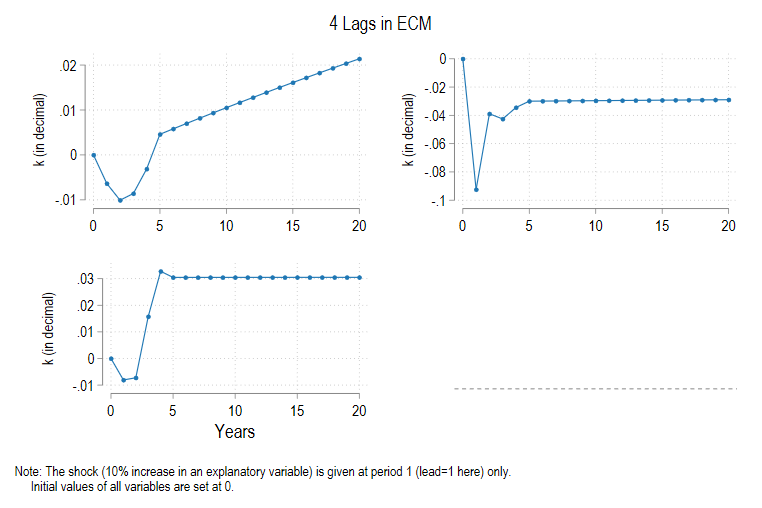
\includegraphics[width=.75\linewidth]{_fig/FImpulseResposne.png}
    \captionsetup{width=0.80\textwidth}
    \caption{
     This chart shows the impulse response functions for all estimated variables.}
\end{figure}
\clearpage

\subsection{Frequency of Borrowing}

One striking aspect of the debt data for school districts is that there is a wide variation in the frequency with which districts borrow for their capital expenditures. In theory, the frequency of debt would be expected to have no impact at all on the level of investment in new capital. This is because districts have accounts called bond funds, which provide a mechanism by which borrowed funds can be stored and segmented from current accounts. Districts that borrow with bonds will face larger fixed costs than those using bank financing, so it might be expected that larger districts using bond finance would borrow less frequently than those using bank finance. The use of bond funds by districts borrowing with bonds would nonetheless allow investment to occur at an identical rate as a district using bank financing. 

Some school districts do not borrow to finance their capital expenditures, rather they finance capital out of current resources. Again, borrowing would not be expected to impact the level of capital outside of small wealth effects. Districts that finance capital using current resources would presumably have started building their capital with a lag, but outside of the initial effects current finance of investment would be expected to approximate debt service (principal plus interest), and thus the level of capital should again be independent of the financing source.

Based on the above reasoning, we estimate the ECM by segmenting districts based on the frequency with which they borrow. To investigate whether administrative procedures impact investment in capital, we segment our panel data between districts that borrow more than about 13 times over our 40 year sample, or less. It appears to be true that school districts that borrow more frequently borrow less each time than school districts that borrow infrequently (with a small effect on total debt per capita). 

We expect to further cement the administrative definitions of newly issued debt in future versions of this research. If administrative procedures are correlated with capital stock, it would indicate either implicit shadow prices that affect investment, or it would indicate discontinuities in information would permit administrators to pursue different investment paths.

The ECM estimates in Table show estimation for how the ln of the Capital Stock varies with school district per capita income, population, and enrollment. Table shows the same specification for school districts that borrow more frequently. Low frequency borrowers tend to have higher enrollments. Despite that, investment per student, debt per student, capital stock per student, and debt newly issued per student are all larger for the districts that borrow frequently. Further, as we see from the estimates below, there are significant differences in the ECM estimates.

\begingroup
\singlespacing
\begin{table}[H] % Allow to float to top/bottom
    \centering
    \begin{tabular}{lcc}
\hline
 & Log of Capital & $\Delta$ Log of Capital \\ 
\hline
lnincomecnty        & 1.052*** &  \\
                    & (0.008)  &  \\
lnenrollment        & -0.142*** &  \\
                    & (0.005)  &  \\
lnpop               & 0.260*** &  \\
                    & (0.008)  &  \\
L.resid             &  & -0.018*** \\
                    &  & (0.001) \\
D.lnincomecnty      &  & -0.048*** \\
                    &  & (0.013) \\
LD.lnincomecnty     &  & -0.048*** \\
                    &  & (0.014) \\
L2D.lnincomecnty    &  & 0.028** \\
                    &  & (0.013) \\
L3D.lnincomecnty    &  & 0.037*** \\
                    &  & (0.014) \\
L4D.lnincomecnty    &  & 0.061*** \\
                    &  & (0.013) \\
LD.lncapital        &  & 0.444*** \\
                    &  & (0.005) \\
L2D.lncapital       &  & -0.120*** \\
                    &  & (0.005) \\
L3D.lncapital       &  & 0.005 \\
                    &  & (0.005) \\
L4D.lncapital       &  & -0.025*** \\
                    &  & (0.005) \\
D.lnenrollment      &  & -0.912*** \\
                    &  & (0.007) \\
LD.lnenrollment     &  & 0.537*** \\
                    &  & (0.008) \\
L2D.lnenrollment    &  & -0.027*** \\
                    &  & (0.008) \\
L3D.lnenrollment    &  & 0.080*** \\
                    &  & (0.008) \\
L4D.lnenrollment    &  & 0.034*** \\
                    &  & (0.008) \\
D.lnpop             &  & -0.060 \\
                    &  & (0.055) \\
LD.lnpop            &  & 0.010 \\
                    &  & (0.068) \\
L2D.lnpop           &  & 0.274*** \\
                    &  & (0.065) \\
L3D.lnpop           &  & 0.192*** \\
                    &  & (0.063) \\
L4D.lnpop           &  & -0.040 \\
                    &  & (0.049) \\
\hline
School Districts    & 1330 & \\
Observations        & 53200 & 46550 \\
\hline
\end{tabular}
\caption{Regression Results: Log of Capital and Change in Log of Capital (Alternative Sample)}


\end{table}
\endgroup
 
\begingroup
\singlespacing
\begin{table}[H]
    \centering
    \begin{tabular}{lcc}
\hline
 & Log of Capital & $\Delta$ Log of Capital \\ 
\hline
lnincomecnty        & 1.179*** &  \\
                    & (0.009)  &  \\
lnenrollment        & -0.367*** &  \\
                    & (0.007)  &  \\
lnpop               & 0.386*** &  \\
                    & (0.011)  &  \\
L.resid             &  & -0.007*** \\
                    &  & (0.000) \\
D.lnincomecnty      &  & -0.081*** \\
                    &  & (0.015) \\
LD.lnincomecnty     &  & -0.058*** \\
                    &  & (0.015) \\
L2D.lnincomecnty    &  & -0.037** \\
                    &  & (0.015) \\
L3D.lnincomecnty    &  & 0.040*** \\
                    &  & (0.015) \\
L4D.lnincomecnty    &  & 0.065*** \\
                    &  & (0.015) \\
LD.lncapital        &  & 0.474*** \\
                    &  & (0.005) \\
L2D.lncapital       &  & -0.107*** \\
                    &  & (0.005) \\
L3D.lncapital       &  & 0.003 \\
                    &  & (0.005) \\
L4D.lncapital       &  & -0.022*** \\
                    &  & (0.005) \\
D.lnenrollment      &  & -0.937*** \\
                    &  & (0.009) \\
LD.lnenrollment     &  & 0.497*** \\
                    &  & (0.010) \\
L2D.lnenrollment    &  & -0.058*** \\
                    &  & (0.010) \\
L3D.lnenrollment    &  & 0.084*** \\
                    &  & (0.010) \\
L4D.lnenrollment    &  & 0.062*** \\
                    &  & (0.009) \\
D.lnpop             &  & -0.072 \\
                    &  & (0.073) \\
LD.lnpop            &  & -0.055 \\
                    &  & (0.092) \\
L2D.lnpop           &  & 0.116 \\
                    &  & (0.091) \\
L3D.lnpop           &  & 0.139 \\
                    &  & (0.090) \\
L4D.lnpop           &  & 0.068 \\
                    &  & (0.068) \\
\hline
School Districts    & 1279 & \\
Observations        & 51160 & 44765 \\
\hline
\end{tabular}

\end{table}
\endgroup

\clearpage

The response of capital to enrollment, income per capita and population is statistically lower in the high frequency sample than the low frequency of borrowing. This result seems a bit counter-intuitive, although it may reflect that high frequency borrowers are more likely to utilize commercial banks rather than issue bonds. 

To fully appreciate the difference in the two samples, however, we show the impulse response functions for an income shock in Figure 6 below:

As with the impulse response for the full sample, we see an assumed increase in income of 10\% stimulates capital, but only very slowly does the capital stock move towards long run steady state. What is interesting in the sample split, however, is that the high frequency borrowers, while starting at the same place, move much more quickly to steady state than do the low frequency borrowers. This is true despite that the two samples have very similar steady state values, as shown in the dotted line at the top.

Splitting the sample by borrowing frequency is somewhat more consequential in the impulse response functions for enrollment. Figure 7 shows:

Here the steady state value is lower for the Low Frequency sample than the High Frequency sample. Despite that difference, the transition path for both samples is similar. The striking difference, however, is that the Low Frequency sample gets much closer to the steady state than does the High Frequency sample. This result is again despite the similarity in the transition path in the two samples.

\section{Instrument Variable Approach}

In order to find a causal relationship, instrument enrollment, population and income per capita with x, y, and z.

\section{Summary and Conclusions}

This paper has examined capital expenditures by K-12 school districts, to determine whether they are focused on students, or if there may be other elements that motivate capital spending. The purpose underlying our examination is recent attempts to estimate the rate of return to capital in education (***cite). If school districts are motivated by other criteria that simply students, then estimating the impact of capital on test score (or other student achievement) outputs is problematic, because it is unlikely the school districts will be on their production frontier.

Our examination is over five questions. The first two involve simply the data means. We ask whether there is basic evidence that capital spending is smoothed to a greater extent than is current spending. We do not find even as much evidence as exists for current spending that local governments smooth. This is true looking at the standard deviation of investment over time, and looking at the level of bond funds (borrowed money available to be spent on capital). Additionally, there is a high degree of heterogeneity in how school districts appear to manage their capital financing, suggesting there is not a systematic approach to this important element of school district finances.

The other approach we use to answer the remaining three questions is to estimate an Error Correction Model for annual capital investment. Estimation over our panel data for 2609 districts over 40 years finds that enrollment is much less important than two elements describing the tax base; population, and per capita income. This finding is more consistent with a budget maximization model than one where capital spending is motivated by students. We further find that the speed of adjustment is extremely slow, yet faster for the tax base variables than enrollment. The final test is to segment the data by school districts that frequently borrow compared to rarely borrow. Because school districts have dedicated bond funds, borrowing frequency should be orthogonal to the level of investment, or capital. We find that, however, frequent borrowers have higher capital levels, and somewhat different paths of adjustment than infrequent borrowers.

This preliminary examination has found that it appears unlikely in the extreme that school districts are on the production frontier for capital. Thus, general analyses of capital are unlikely to discover the true shape of the education production function with respect to capital. It also appears that school district officials probably need some general training for how to manage capital expenditures, since heterogeneity appears much larger than suggested by institutional variety.
